
%
%  $Description: Author guidelines and sample document in LaTeX 2.09$ 
%
%  $Author: ienne $
%  $Date: 1995/09/15 15:20:59 $
%  $Revision: 1.4 $
%

\documentclass[times, 10pt,twocolumn]{article} 
\usepackage{paper}
\usepackage{times}
\usepackage{graphicx}
\usepackage{float}
\usepackage{amsmath}

%\documentstyle[times,art10,twocolumn,latex8]{article}

%------------------------------------------------------------------------- 
% take the % away on next line to produce the final camera-ready version 
% \pagestyle{empty}

%------------------------------------------------------------------------- 
\begin{document}

\title{18-752 Final Project Report: EMG Signal Classification}

\author{Paul Griffioen\\Dept. of Electrical and Computer Engineering\\Carnegie Mellon University\\ pgriffi1@andrew.cmu.edu\\
% For a paper whose authors are all at the same institution, 
% omit the following lines up until the closing ``}''.
% Additional authors and addresses can be added with ``\and'', 
% just like the second author.
\and
Thomas Mayo-Smith\\Dept. of Electrical and Computer Engineering\\Carnegie Mellon University\\tmayosmi@andrew.cmu.edu\\
}

\maketitle
\thispagestyle{empty}

%------------------------------------------------------------------------- 
\begin{abstract}
The main objective of this project is to improve upon the existing method of EMG signal classification used by the software package CAPS by improving classification accuracy and latency. To achieve this objective, a gaussian mixture model (GMM) is used to perform blind identification and detection on a novel data set collected using CAPS. Using the labels generated by the GMM, an exponential model with a categorical prior is used for supervised identification and detection. Both methods very clearly classify EMG samples more accurately than CAPS, but only the GMM is fully capable of reducing classification latency. Additionally, the optimal number of channels used in identification and detection for both methods is explored.
\end{abstract}

%------------------------------------------------------------------------- 
\section{Introduction and Motivation}
It has been widely reported that prosthesis patients abandon advanced prosthetic limbs capable of being controlled via EMG signals as a result of having too much difficulty learning how to isolate their muscle contractions in a way which prosthetic limbs can understand them. To alleviate this frustration, special games controlled via EMG signals have been developed to make pre-prosthetic training more effective. Unfortunately the method used by the existing software package which classifies EMG signals during gameplay is inaccurate and irritating to use. This work explores the ability of a GMM and an exponential distribution with a categorical prior to classify EMG signals as game actions. In particular the game used in experiments is Space Invaders$^{\tiny{\textregistered}}$, and EMG signals produced when a player is flexing, extending, co-contracting, and resting his or her forearm are classified as "move left", "move right", "shoot", and "do nothing" respectively. The results show that our proposed methods of EMG signal classification are advantageous to use over the existing one as a result of their lower classification latency and better ability to cluster different types of EMG signals.

%------------------------------------------------------------------------- 
\section{Data Set Collection}
Using a custom sleeve lined with 8 EMG electrodes that sample at 100 Hz, the software package CAPS was used to record 2 games of Space Invaders$^{\tiny{\textregistered}}$ (Figure \ref{data_collection}). Each EMG sample consists of a vector of 9 values. The first value corresponds to the classification label determined by the CAPS software, and the next 8 values correspond to the absolute values of the electrograms read from the 8 EMG electrodes at a particular point during the game. CAPS only uses sample values from channels 1 and 4 to make a classification because these channels are on opposite sides of the forearm muscle and are thus best suited to distinguish between the muscle contractions a player performs during Space Invaders$^{\tiny{\textregistered}}$ gameplay. By observing histograms of sample values from each channel, it is clear channels other than 1 and 4 correspond to muscles not used very much during gameplay (Figure \ref{histogram}). The histograms of these other channels tend to be noisy and similar across contractions. CAPS claims in its documentation to make classifications using a simple threshold method. However, this is not clearly observed in the collected data likely due to noise and imprecise hardware measurements (Figure \ref{caps_clusters}). As a result, the data was reclassified by manually implementing a threshold method (Figure \ref{manual_clusters}). Limits of this classification method are clearly illustrated in Figure \ref{manual_clusters_fail}.

%------------------------------------------------------------------------- 
\section{Blind Identification and Detection}
The first strategy used to improve EMG signal classification is a GMM for blind Identification and detection. The GMM is composed of 4 bivariate gaussians, each of which has parameters with a categorical distribution. Each gaussian is intended to fit the EMG data corresponding to each contraction, and the dimensions of each gaussian correspond to the number of channels being used for classification (in this case 2). The categorical prior corresponds to the likelihood of a particular contraction during gameplay. Equations 1-5 summarize this GMM model.
\begin{equation}
\mathbf{x} = \text{EMG sample}
\end{equation}
\begin{equation}
\lambda_i = \text{contraction }i, i\in[1,2,3,4]
\end{equation}
\begin{equation}
f_{\mathbf{\mu_i},\mathbf{\sigma_i^2}}(\mathbf{x}|\lambda_i) = \mathcal{N}(\mathbf{\mu_i},\mathbf{\sigma_i^2})
\end{equation}
\begin{equation}
f_{p_i}(\lambda) = \text{categorical density with parameters } p_i
\end{equation}
\begin{equation}
f(\mathbf{x}) = \sum_{i=1}^{4}f_{p_i}(\lambda_i)f_{\mathbf{\mu_i},\mathbf{\sigma_i^2}}(\mathbf{x}|\lambda_i)
\end{equation}

The maximum likelihood estimate (MLE) of the GMM parameters can be solved via equations 6-9.
\begin{equation}
\begin{split}
L(\mathbf{\mu},\mathbf{\sigma^2}, p, \lambda, \mathbf{X}) & = \log{f_{\mathbf{\mu},\mathbf{\sigma^2},p}(\mathbf{X})} \\
& = \sum_{k=1}^{n}\log{\sum_{i=1}^{4}f_{\mathbf{\mu_i},\mathbf{\sigma_i^2}}(\mathbf{x_k}|\lambda_i)f_{p_i}(\lambda_i)}
\end{split}
\end{equation}
\begin{equation}
\frac{\partial}{\partial{\mathbf{\mu}}}L(\mathbf{\mu},\mathbf{\sigma^2}, p, \lambda, \mathbf{X}) = 0 \text{ } => \text{ } \mathbf{\hat{\mu}}
\end{equation}
\begin{equation}
\frac{\partial}{\partial{\mathbf{\sigma^2}}}L(\mathbf{\mu},\mathbf{\sigma^2}, p, \lambda, \mathbf{X}) = 0 \text{ } => \text{ } \mathbf{\hat{\sigma}^2}
\end{equation}
\begin{equation}
\frac{\partial}{\partial{p}}L(\mathbf{\mu},\mathbf{\sigma^2}, p, \lambda, \mathbf{X}) = 0 \text{ } => \text{ } \hat{p}
\end{equation}

There is no closed form solution to calculate the MLE of the GMM parameters. Solving numerically via Newton's method or gradient decent is slow so the Expectation Maximization (EM) algorithm is used. The GMM parameters are initialized using the data which is poorly labeled by the threshold method. For instance, the initial mean of the gaussian which is expected to eventually fit flexion samples is initialized to the mean of the data points labeled flexion by the threshold method. Initializing parameters this way eliminates the need to take additional steps to determine which gaussian corresponds to a particular contraction type after the GMM parameters have converged. Equations 10-13 summarize the EM algorithm used.\\

Expectation Step
\begin{equation}
f_{\mathbf{\hat{\mu}_i},\mathbf{\hat{\sigma}_i^2},\hat{p_i}}(\lambda_i|\mathbf{x}) = \frac{f_{\hat{p_i}}(\lambda_i)f_{\mathbf{\hat{\mu}_i},\mathbf{\hat{\sigma}_i^2}}(\mathbf{x}|\lambda_i)}{\sum_{i=1}^{4}f_{\hat{p_i}}(\lambda_i)f_{\mathbf{\hat{\mu}_i},\mathbf{\hat{\sigma}_i^2}}(\mathbf{x}|\lambda_i)}
\end{equation}

Maximization Step
\begin{equation}
f_{\mathbf{\mu_i},\mathbf{\sigma_i^2},p_i}(\lambda_i|\mathbf{x}) = \frac{1}{n}\sum_{k=1}^{n}f_{\mathbf{\hat{\mu}_i},\mathbf{\hat{\sigma}_i^2}}(\lambda_i|\mathbf{x_k})
\end{equation}
\begin{equation}
\mathbf{\mu_i} = \frac{\sum_{k=1}^{n}f_{\mathbf{\hat{\mu}_i},\mathbf{\hat{\sigma}_i^2},\hat{p_i}}(\lambda_i|\mathbf{x_k})\mathbf{x_k}}{\sum_{k=1}^{n}f_{\mathbf{\hat{\mu}_i},\mathbf{\hat{\sigma}_i^2},\hat{p_i}}(\lambda_i|\mathbf{x_k})}
\end{equation}
\begin{equation}
\mathbf{\sigma_i^2} = \frac{\sum_{k=1}^{n}f_{\mathbf{\hat{\mu}_i},\mathbf{\hat{\sigma}_i^2},\hat{p_i}}(\lambda_i|\mathbf{x_k})(\mathbf{x_k}-\mathbf{\mu_i})(\mathbf{x_k}-\mathbf{\mu_i})^\text{T}}{\sum_{k=1}^{n}f_{\mathbf{\hat{\mu}_i},\mathbf{\hat{\sigma}_i^2},\hat{p_i}}(\lambda_i|\mathbf{x_k})}
\end{equation}

The EM algorithm is set to stop iterating after a maximum of 1000 iterations or if the maximum update to a particular parameter is less than 0.01. Once the parameters of the GMM are estimated, a maximum a posteriori probability (MAP) detector is used to classify the EMG samples via Equation 14. Results for this method can be seen in Figures \ref{gmm_clusters}, \ref{posterior_probabilities}, and \ref{posterior_probabilities_close_up}.
\begin{equation}
\hat{\lambda} = \max_{i}f_{\mathbf{\mu_i},\mathbf{\sigma_i^2},p_i}(\lambda_i|\mathbf{x})
\end{equation}

%------------------------------------------------------------------------- 
\section{Supervised Identification and Detection}

The other method used to improve EMG signal classification is supervised identification and detection. The parameters for a given labeled data set are first identified, and then that identified model is used for detection where unlabeled data is classified according to a MAP detector. As is shown in Equations 15 and 16, each EMG sample in the given data set has an associated label that represents the contraction type.
\begin{equation}
\mathbf{x} = \text{EMG sample}
\end{equation}
\begin{equation}
\lambda_i = \text{contraction }i, i\in[1,2,3,4]
\end{equation}

Equation 17 shows how an exponential model is used with the labeled data set, and as discussed earlier, the histogram in Figure \ref{histogram} demonstrates why an exponential model is used. The subscript $ch$ represents the channel of the EMG sample.
\begin{equation}
f_{\theta_{i_{ch}}}(x_{ch}|\lambda_i) = \theta_{i_{ch}}\mathrm{e}^{-\theta_{i_{ch}}x_{ch}}
\end{equation}

Equation 18 demonstrates how a categorical prior is used to model the distribution of the contractions. This specific categorical prior is chosen because it is the MLE of $f(\lambda_i)$.
\begin{equation}
f(\lambda_i) = \frac{\text{\# data points for }\lambda_i}{\text{total \# of labeled data points}}
\end{equation}

Equations 19-20 depict how the log-likelihood function is used to calculate the MLE of the exponential model given the labeled data set. A Naive Bayes model is used in that each $f_{\theta_{i_{ch}}}(x_{ch}|\lambda_i)$ is assumed to be independent.
\begin{equation}
\begin{split}
L(\theta_{i_{ch}},\lambda_i,X_{ch}) & = \log{f_{\theta_{i_{ch}}}(X_{ch}|\lambda_i)} \\
& = \log{\prod_{k=1}^{n}f_{\theta_{i_{ch}}}(x_{k_{ch}}|\lambda_i)} \\
& = \sum_{k=1}^{n}\log{f_{\theta_{i_{ch}}}(x_{k_{ch}}|\lambda_i)}
\end{split}
\end{equation}
\begin{equation}
\frac{\partial}{\partial{\theta_{i_{ch}}}}L(\theta_{i_{ch}},\lambda_i,X_{ch}) = 0 \text{ } => \text{ } \hat{\theta}_{i_{ch}} = \frac{n}{\sum_{k=1}^{n}x_{k_{ch}}}
\end{equation}

Equations 21-22 show how a MAP detector is used to classify the EMG samples. Given an EMG sample, $i$ is chosen such that the probability of $\lambda_i$ is greater than the probability of any other $\lambda_i$.
\begin{equation}
f_{\theta_i}(\lambda_i|\mathbf{x}) = \frac{f(\lambda_i)\prod_{\text{ch}}f_{\theta_{i_{ch}}}(x_{ch}|\lambda_i)}{\sum_{i=1}^{4}f(\lambda_i)\prod_{\text{ch}}f_{\theta_{i_{ch}}}(x_{ch}|\lambda_i)}
\end{equation}
\begin{equation}
\hat{\lambda} = \max_{i}f_{\theta_i}(\lambda_i|\mathbf{x})
\end{equation}

Results for this method can be seen in Figures \ref{expCAPS} and \ref{expGMM}. Additionally, Figures \ref{expCAPSall}, \ref{expGMMall}, and \ref{GMMall} demonstrate how important all the channels are in classifying an EMG sample as opposed to only using channels 1 and 4.

%------------------------------------------------------------------------- 
%\nocite{ex1,ex2}
%\bibliographystyle{paper}
%\bibliography{paper}
%
%%\begin{thebibliography}{}
%\begin{thebibliography}{}\setlength{\itemsep}{-1ex}\small
%
%\bibitem{incentives}
%Author. "Title." \textit{Journal}, pp. \#-\#, Year.
%
%\end{thebibliography}

\section*{Appendix}

\begin{figure}[h]
  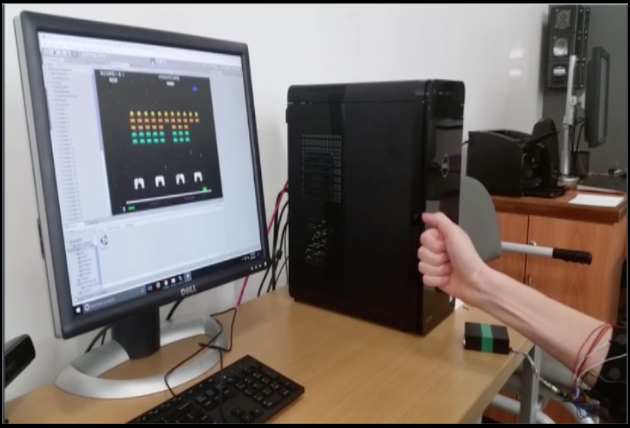
\includegraphics[width=\linewidth]{Figures/f1.png}
  \caption{Data Collection.}
  \label{data_collection}
\end{figure}

\begin{figure}[h]
  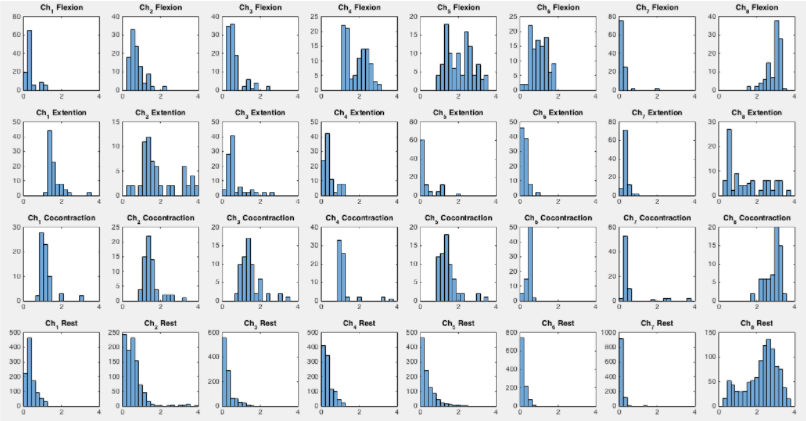
\includegraphics[width=\linewidth]{Figures/f2.png}
  \caption{Each histogram ${i,j}$ shows the distribution of EMG samples for contraction $i$ and channel $j$.}
  \label{histogram}
\end{figure}

\begin{figure}[h]
  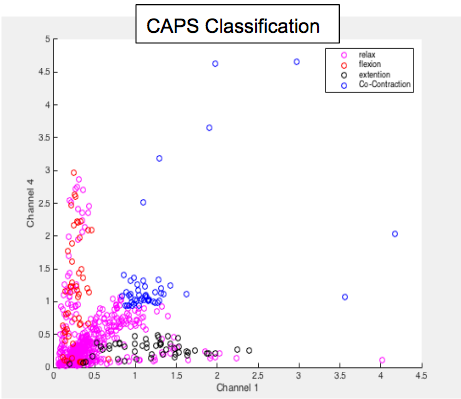
\includegraphics[width=\linewidth]{Figures/f3.png}
  \caption{Contraction clusters determined by the CAPS software. CAPS only uses electrogram values from channel 1 and channel 4 for classification.}
  \label{caps_clusters}
\end{figure}

\begin{figure}[h]
  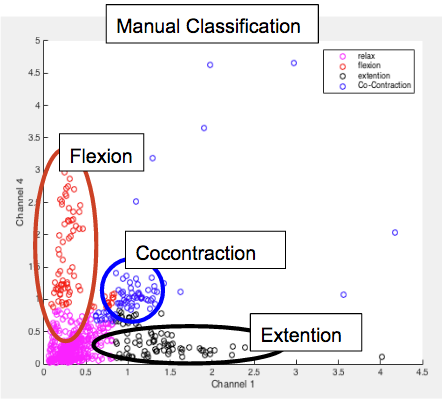
\includegraphics[width=\linewidth]{Figures/f4.png}
  \caption{Contraction clusters determined by the manually implemented CAPS algorithm.}
  \label{manual_clusters}
\end{figure}

\begin{figure}[h]
  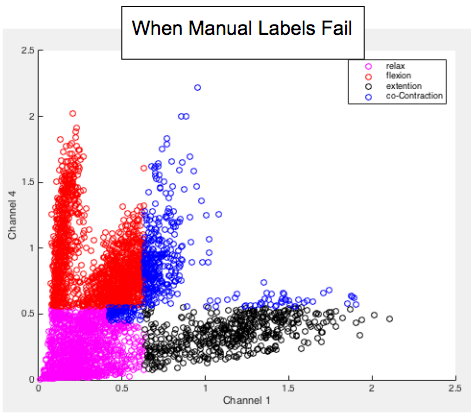
\includegraphics[width=\linewidth]{Figures/f5.png}
  \caption{Linear decision boundaries of the CAPS algorithm are not appropriate for classification.}
  \label{manual_clusters_fail}
\end{figure}

\begin{figure}[h]
  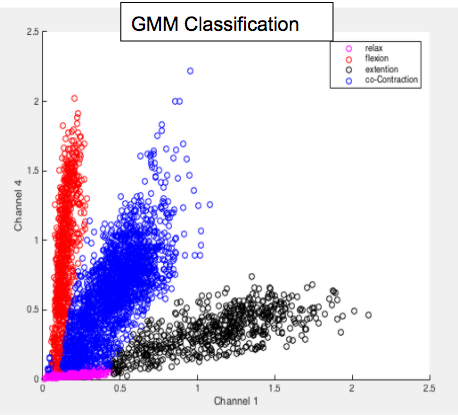
\includegraphics[width=\linewidth]{Figures/f6.png}
  \caption{Contraction clusters determined by the GMM.}
  \label{gmm_clusters}
\end{figure}

\begin{figure}[h]
  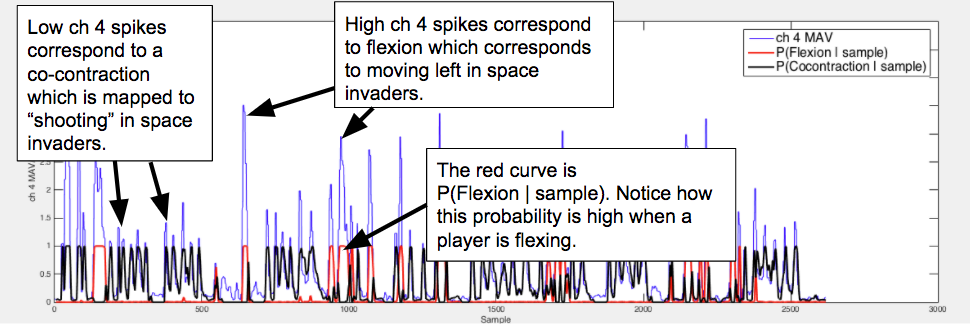
\includegraphics[width=\linewidth]{Figures/f7.png}
  \caption{Posterior probabilities of flexion and co-contraction overlaid on top of the channel 4 EMG signal.}
  \label{posterior_probabilities}
\end{figure}

\begin{figure}[h]
  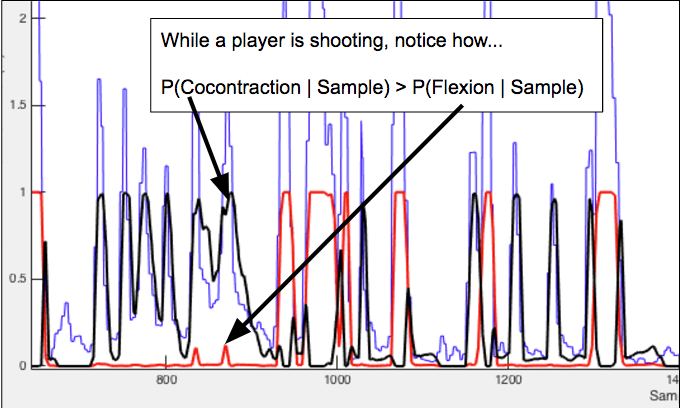
\includegraphics[width=\linewidth]{Figures/f8.png}
  \caption{Close-up of Figure 7.}
  \label{posterior_probabilities_close_up}
\end{figure}

\begin{figure}[h]
  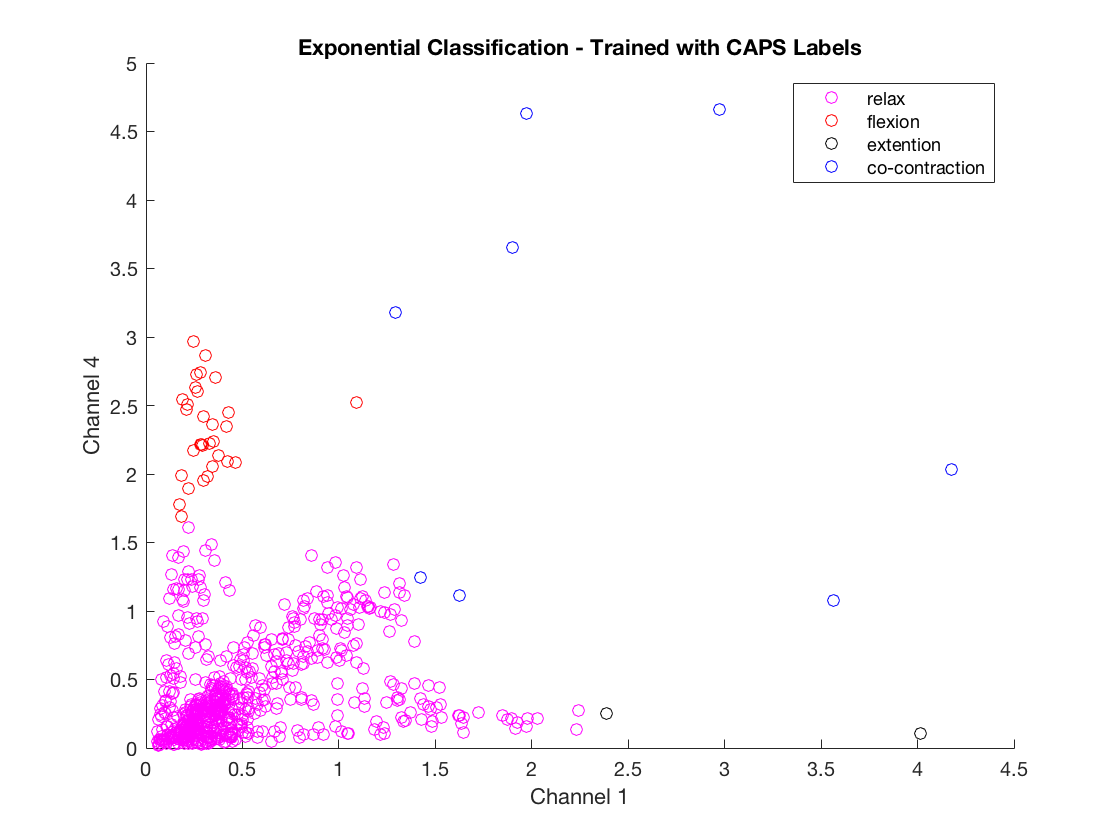
\includegraphics[width=\linewidth]{Figures/f9.png}
  \caption{Poor exponential classification using CAPS labels (accuracy: 85.17\%).}
  \label{expCAPS}
\end{figure}

\begin{figure}[h]
  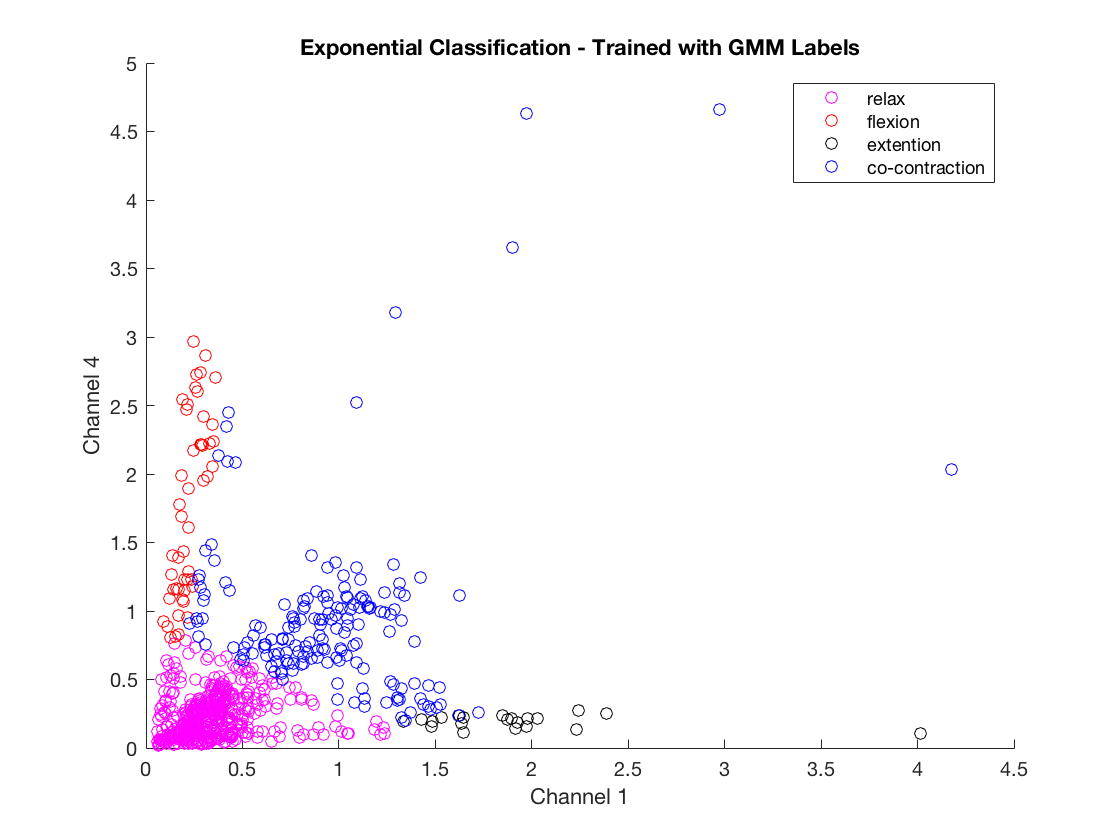
\includegraphics[width=\linewidth]{Figures/f10.png}
  \caption{Better exponential classification using GMM labels (accuracy: 83.18\%).}
  \label{expGMM}
\end{figure}

\begin{figure}[h]
  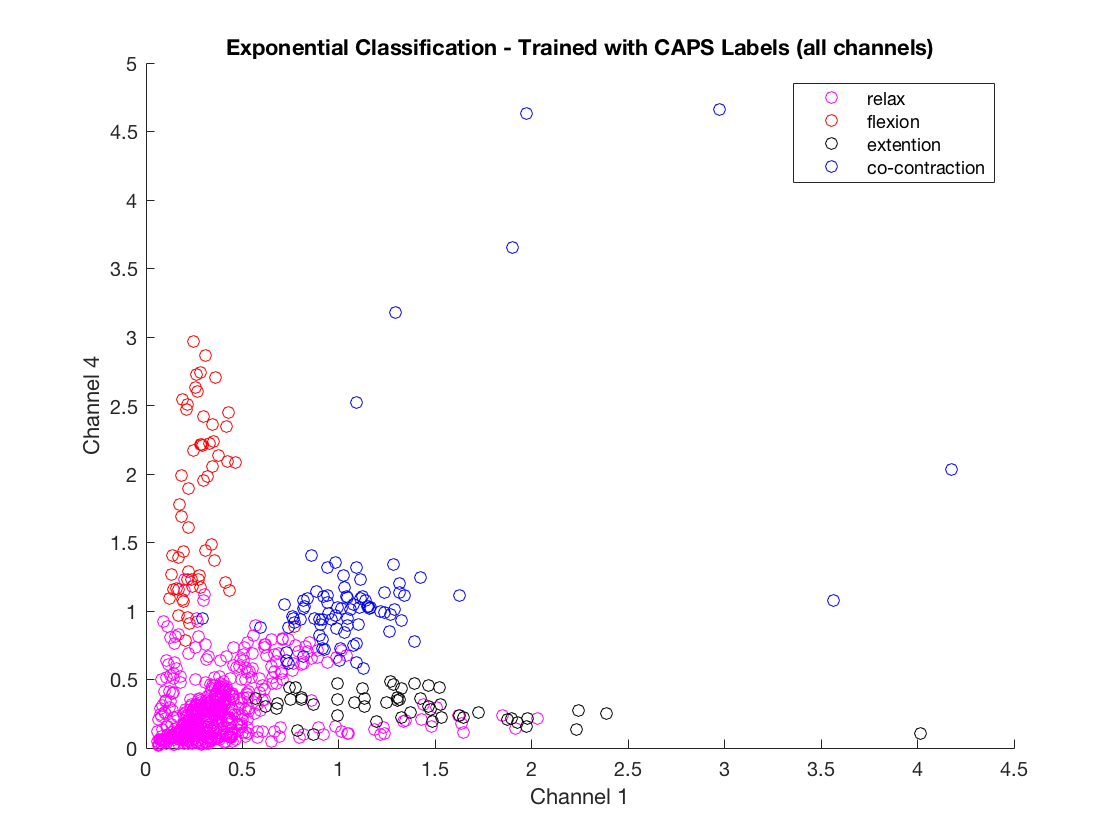
\includegraphics[width=\linewidth]{Figures/f11.png}
  \caption{Exponential classification using all channels improves clustering with CAPS labels (accuracy: 86.93\%).}
  \label{expCAPSall}
\end{figure}

\begin{figure}[h]
  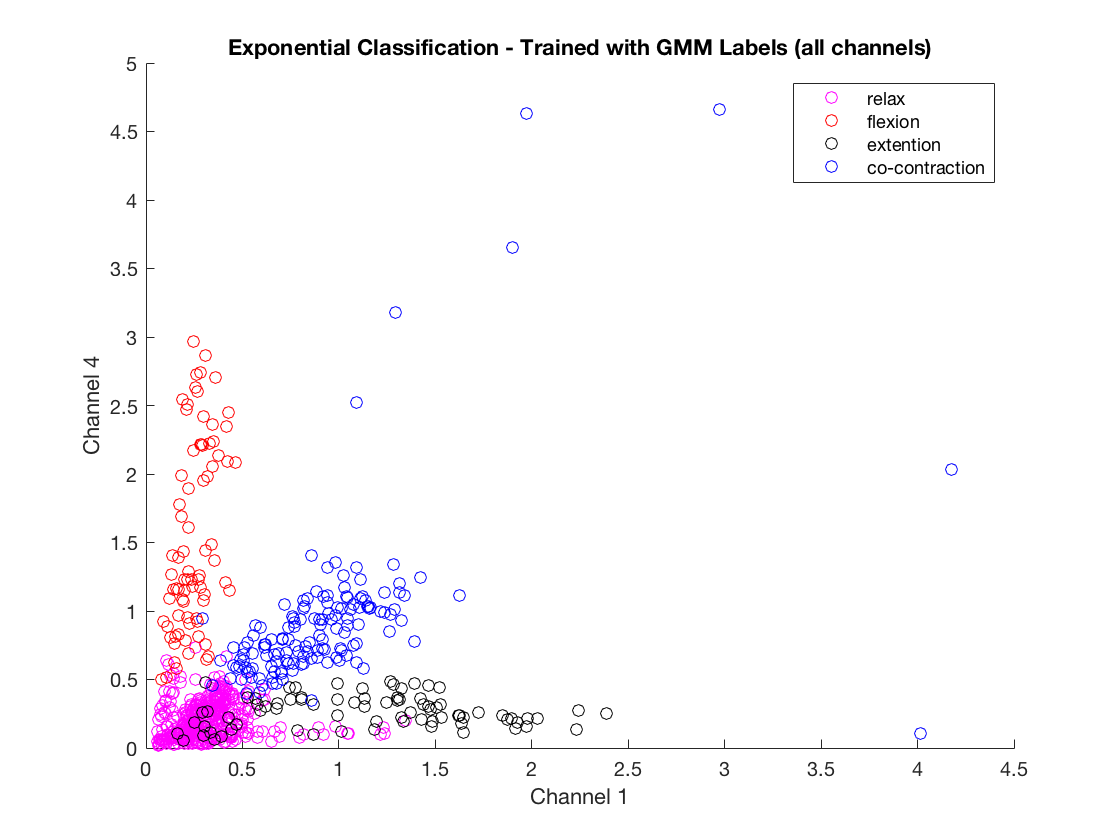
\includegraphics[width=\linewidth]{Figures/f12.png}
  \caption{Exponential classification using all channels improves clustering with GMM labels (accuracy: 89.83\%).}
  \label{expGMMall}
\end{figure}

\begin{figure}[h]
  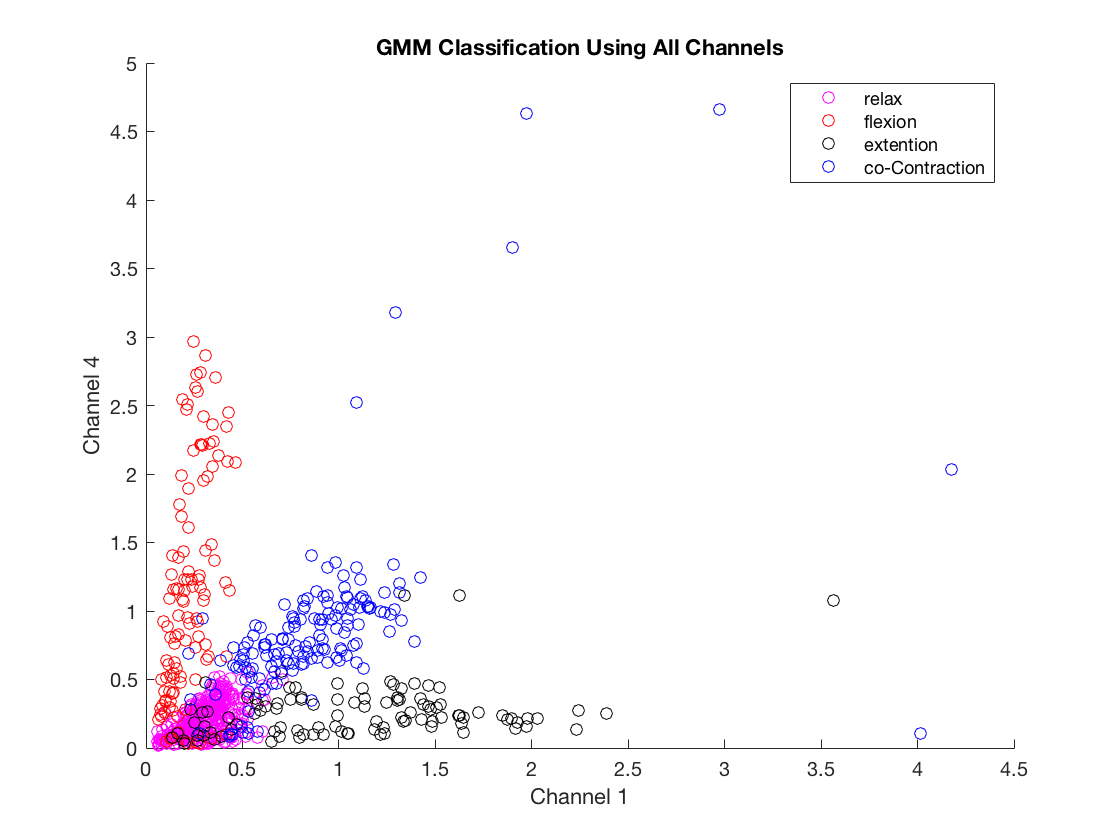
\includegraphics[width=\linewidth]{Figures/f13.png}
  \caption{GMM classification using all channels weakens clustering (compared with Figure 6).}
  \label{GMMall}
\end{figure}

\end{document}
